\documentclass[a4paper,12pt,obeyspaces,spaces,hyphens]{article}

\usepackage{agenda}
\usepackage{colortbl}
\usepackage{xcolor}
\usepackage{calc}

\hypersetup{pdftitle={Boot time optimization training},
  pdfauthor={Bootlin}}

\renewcommand{\arraystretch}{2.0}

\begin{document}

\setlength{\arrayrulewidth}{0.8pt}

\begin{center}
\LARGE
Boot Time Optimization Training\\
\large
3-day session
\end{center}
\vspace{1cm}

\small
\newcolumntype{g}{>{\columncolor{fedarkblue}}m{4cm}}
\newcolumntype{h}{>{\columncolor{felightblue}}X}

\arrayrulecolor{lightgray} {
  \setlist[1]{itemsep=-5pt}
  \begin{tabularx}{\textwidth}{|g|h|}
    {\bf Title} & {\bf Boot Time Optimization Training}\\
    \hline

    {\bf Overview} &
    Measuring boot time \par
    Reducing user space boot time \par
    Reducing kernel boot time \par
    Bootloader optimizations \par
    Advanced techniques and alternatives \par
    Practical labs with the ARM-based BeagleBone Black board
    (or with its Wireless variant).\\
    \hline
    {\bf Materials} &
    Check that the course contents correspond to your needs:
    \newline \url{https://bootlin.com/doc/training/boot-time}. \\
    \hline

    {\bf Duration} & {\bf Three} days - 24 hours.
    \newline 25\% of lectures, 75\% of practical labs. \\
    \hline

    {\bf Trainer} & One of the engineers listed on
    \newline \url{https://bootlin.com/training/trainers/}\\
    \hline

    {\bf Language} & Oral lectures: English or French.
    \newline Materials: English.\\
    \hline

    {\bf Audience} & People developing embedded Linux systems.
    \newline People supporting embedded Linux system developers. \\
    \hline

    {\bf Prerequisites} & {\bf Knowledge and practice of UNIX or
      GNU/Linux commands}
    \newline People lacking experience on this topic should get
    trained by themselves, for example with our freely available
    on-line slides:
    \newline \url{https://bootlin.com/blog/command-line/} \vspace{1em}
    \newline {\bf Knowledge and practice of embedded Linux system
    development} \\
    \hline
  \end{tabularx}

  \begin{tabularx}{\textwidth}{|g|h|}
    {\bf Required equipment} &
    {\bf For on-site sessions only.}
    \newline Everything is supplied by Bootlin in public sessions.
    \begin{itemize}
    \item Video projector
    \item PC computers with at least 8 GB of RAM, and Ubuntu Linux
    installed in a {\bf free partition of at least 30 GB. Using Linux
      in a virtual machine is not supported}, because of issues
    connecting to real hardware.
    \item We need Ubuntu Desktop 20.04 (Xubuntu and other
    variants are fine). We don't support other
    distributions, because we can't test all possible package versions.
    \item {\bf Connection to the Internet} (direct or through the
    company proxy).
    \item {\bf PC computers with valuable data must be backed up}
    before being used in our sessions.  Some people have already made
    mistakes during our sessions and damaged work data.
    \end{itemize}\\
    \hline

    {\bf Materials} & Electronic copies of presentations and
    labs.
    \newline Electronic copy of lab files.\\
    \hline

\end{tabularx}}
\normalsize

\feagendatwocolumn
{Hardware}
{
  The hardware platform used for the practical labs of this training
  session is the {\bf BeagleBone Black} board, which features:

  \begin{itemize}
  \item An ARM AM335x processor from Texas Instruments (Cortex-A8
    based), 3D acceleration, etc.
  \item 512 MB of RAM
  \item 2 GB of on-board eMMC storage
        \newline(4 GB in Rev C)
  \item USB host and device
  \item HDMI output
  \item 2 x 46 pins headers, to access UARTs, SPI buses, I2C buses
    and more.
  \end{itemize}
}
{}
{
  \begin{center}
    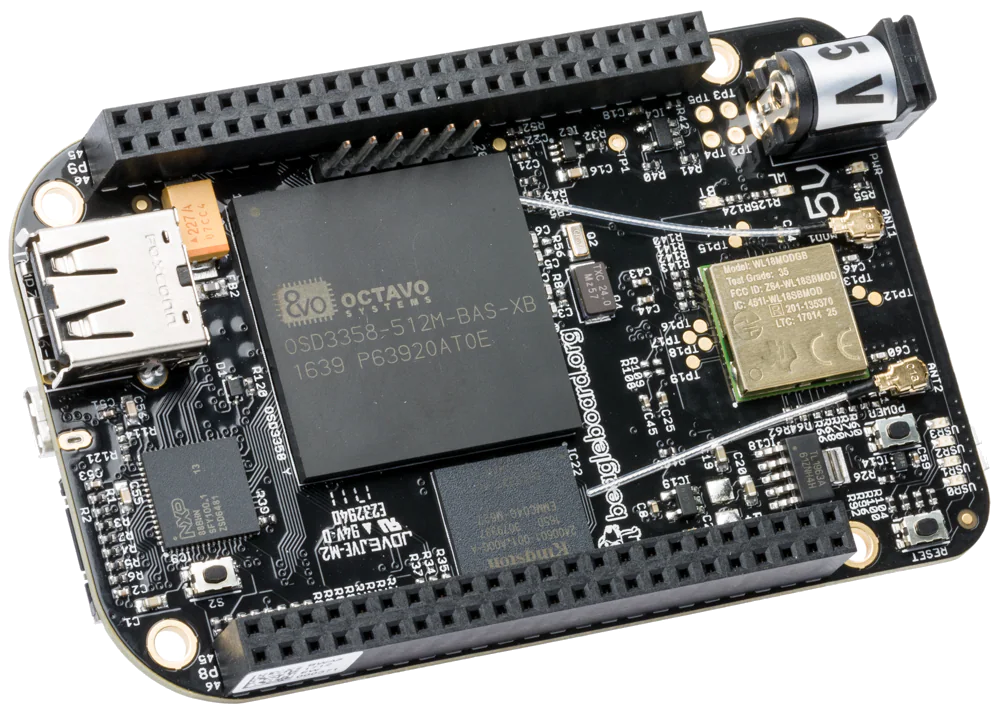
\includegraphics[height=5cm]{../slides/beagleboneblack-board/beagleboneblack.png}
  \end{center}
}

\feagendaonecolumn
{Practical labs}
{
  The practical labs of this training session use the following
  hardware peripherals:

  \begin{itemize}
  \item A USB webcam
  \item An LCD and touchscreen cape connected to the
    BeagleBone Black board, to display the video captured by the webcam.
  \item We will also use an Arduino board as a way to measure boot time with accurary,
    demonstrating a hardware boot time measurement technique.
  \end{itemize}
}

\section{Day 1 - Morning}

\feagendatwocolumn
{Lecture - Principles}
{
  \begin{itemize}
  \item How to measure boot time
  \item Main ideas
  \end{itemize}
}
{Lab - Preparing the system}
{
 \begin{itemize}
 \item Downloading bootloader, kernel and Buildroot source code
 \item Board setup, setting up serial communication
 \item Configure Buildroot and build the system
 \item Configure and build the U-Boot bootloader. Prepare an SD card
       and boot the bootloader from it.
 \item Configure and build the kernel. Boot the system
 \end{itemize}
}

\section{Day 1 - Afternoon}

\feagendatwocolumn
{Lecture - Measuring time}
{
  \begin{itemize}
  \item Generic software techniques
  \item Hardware techniques
  \item Specific solutions for each stage
  \end{itemize}
}
{Lab - Measuring time - Software solution}
{
 \begin{itemize}
 \item Modify the system to measure time at various steps
 \item Timing messages on the serial console
 \item Timing the execution of the application
 \end{itemize}
}

\feagendatwocolumn
{Lab - Measuring time - Hardware solution}
{
  \begin{itemize}
  \item Measure total boot time by toggling a GPIO
  \item Setting up an Arduino board
  \item Preparing a test circuit with a 7-segment display
  \item Modifying the DTS to configuring Bone Black pins as GPIOs
  \item Making the application drive the custom GPIOs
  \end{itemize}
}
{Lecture - Toolchain optimizations}
{
  \begin{itemize}
  \item Introduction to toolchains
  \item C libraries
  \item Size information
  \item Measuring executable performance with \code{time}
  \end{itemize}
}

\feagendaonecolumn
{Lab - Toolchain optimizations}
{
  \begin{itemize}
  \item Measuring application execution time
  \item Switching to a Thumb2 toolchain
  \item Generate a Buildroot SDK to rebuild faster
  \end{itemize}
}

\section{Day 2- Morning}

\feagendatwocolumn
{Lecture - Application optimization}
{
  \begin{itemize}
  \item Using \code{strace}
  \item Other profiling techniques
  \end{itemize}
}
{Lab - Application optimization}
{
 \begin{itemize}
 \item Finding unnecessary configuration options in applications
 \item Modifying configuration options through Buildroot
 \item Experiments with \code{strace} to trace program execution
 \end{itemize}
}

\feagendatwocolumn
{Lecture - Optimizing system initialization}
{
  \begin{itemize}
  \item Using Bootchart
  \item Optimizing init scripts
  \item Possibility to start your application directly
  \end{itemize}
}
{Lab - Optimizing system initialization}
{
 \begin{itemize}
 \item Using Buildroot to remove unnecessary scripts and commands
 \item Access-time based technique to identify  unused files
 \item Simplifying BusyBox
 \item Starting the application as the init program
 \end{itemize}
}

\section{Day 2 - Afternoon}

\feagendatwocolumn
{Lecture - Filesystem optimizations}
{
  \begin{itemize}
  \item Available filesystems, performance and boot time aspects
  \item Making UBIFS faster
  \item Tweaks for reducing boot time
  \item Booting on an initramfs
  \item Using static executables: licensing constraints
  \end{itemize}
}
{Lab - Filesystem optimizations}
{
 \begin{itemize}
 \item Trying and measuring two block filesystems: ext4 and SquashFS.
 \item Trying and measuring the initramfs solution. Constraints
       due to this solution.
 \end{itemize}
}

\feagendatwocolumn
{Lecture - Kernel optimizations}
{
  \begin{itemize}
  \item Using {\em Initcall debug} to generate a boot graph
  \item Compression and size features
  \item Reducing or suppressing console output
  \item Multiple tweaks to reduce boot time
  \end{itemize}
}
{Lab - Kernel optimizations}
{
 \begin{itemize}
 \item Generating and analyzing a boot graph for the kernel
 \item Find and eliminate unnecessary kernel features
 \item Find the best kernel compression solution for our system
 \end{itemize}
}

\section{Day 3 - Morning}

\feagendaonecolumn
{Lab - Kernel optimizations}
{
 \begin{itemize}
 \item Continued from Day 2
 \end{itemize}
}

\section{Day 3 - Afternoon}

\feagendatwocolumn
{Lecture - Bootloader optimizations}
{
  \begin{itemize}
  \item Compiling U-Boot with fewer features
  \item U-Boot configuration settings that impact boot time
  \item Optimizing kernel loading
  \item Skipping the bootloader - How to modify U-Boot to
        enable its {\em Falcon mode}
  \end{itemize}
}
{Lab - Bootloader optimizations}
{
 \begin{itemize}
 \item Using the above techniques to make the bootloader
    as quick as possible.
 \item Switching to faster storage
 \item Skip the bootloader with U-Boot's {\em Falcon mode}
 \end{itemize}
}

\feagendaonecolumn
{Wrap-up - Achieved results}
{
 \begin{itemize}
 \item Sharing and comparing results achieved by the various groups
 \item Questions and answers, experience sharing with the trainer
 \end{itemize}
}

\end{document}
